We show an approximation preserving reduction from the \ProblemDom{} problem (\ProbDom)
to \ProblemStar{}.
Given an (unweighted) instance of \ProbDom{} $G = (V, E)$ we create an instance of \ProbStar{}
$(G', w)$ where $G' = (L \cup R \cup {c}, E' \cup \{c\} \times L$).
\begin{description}
\item[L] - $\{v_l : v \in V\}$
\item[R] - $\{v_r : v \in V\}$
\item[E'] - $\{u_lv_r : uv \in E\}$
\end{description}
We also set $w(e) = \infty$ for every $e \in E'$ and $w(cv_l) = 1$ for every $v_l \in L$.
Figure~\ref{fig:star-hardness} depicts this transformation.
Clearly the above transformation can be done in polynomial time,
The following two claims show that this is an approximation preserving reduction:

\begin{figure}
\begin{center}
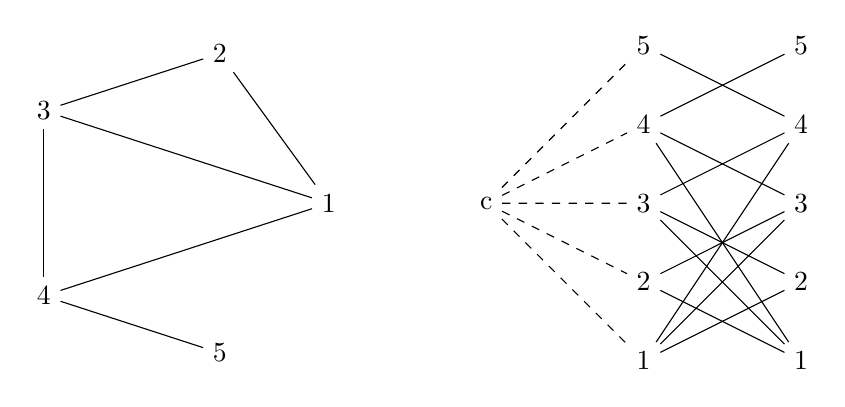
\begin{tikzpicture}[]
\foreach[count=\i] \a in {0,72,...,288}{
	\node(\i) at(\a:2) {\i};
}

\foreach \u \v in {
	1/2,2/3,3/4,4/1,4/5,3/1%
}{
	\draw (\u) -- (\v);
}

\node(c) at(4,0) {c};

\begin{scope}[xshift=6cm, yshift=-3cm]
\foreach \i in {1,...,5}{
	\node(l\i) at(0,\i) {\i};
	\node(r\i) at(2,\i) {\i};
}


\foreach \u \v in {
	1/2,2/3,3/4,4/1,4/5,3/1%
}{
	\draw (l\u) -- (r\v);
	\draw (r\u) -- (l\v);
}

\foreach \i in {1,...,5}{
	\draw[dashed] (c) -- (l\i);
}
\end{scope}
\end{tikzpicture}
\end{center}
\caption{\label{fig:star-hardness}
From left to right:
a) An instance of \ProbDom{} (unweighted graph)
b) The corresponding instance of \ProbStar{}, 
the weight on the original edges (solid black) is infinity 
and the weight on the new edges is 1. 
}
\end{figure} 

\begin{claim}
If $D$ is a dominating set in $G$ then 
$S = (\{c\} \cup \{v_l : v \in D\}, \{cv_l: v \in D\})$ 
is a dominating star in $G'$ that weigh $|D|$. 
\end{claim}

\begin{proof}
$S$ weights $D$ by the definition of $G'$ and $S'$.
Assume for contradiction that it is not a dominating star and let $v$ be a non dominated 
vertex then $v$ is also not dominated in $G$ under $D$ - contradiction.
\end{proof}

\begin{claim}
If $S = (U, F)$ is a dominating star in $G'$ of weight $k < \infty$ 
then $\{v : v_l \in U \setminus \{c\}\}$ is a dominating set in $G$ of size $k$.
\end{claim}

\begin{proof}
Observe that any star that contains more than 3 vertices must be centered at $c$ or otherwise
its weight is infinity.
Thus the leaf of the star dominate all vertices in $R$, by construction, this mean that the
corresponding vertices in the original graph dominate all other vertices.
\end{proof}